\documentclass[a4paper,11pt]{article}

% Packages essentiels
\usepackage[utf8]{inputenc}
\usepackage[T1]{fontenc}
\usepackage{textcomp}   
\usepackage[french]{babel}
\usepackage{amsmath,amssymb,amsfonts}
\usepackage{graphicx}
\usepackage{hyperref}
\usepackage{xcolor}
\usepackage{enumitem}
\usepackage{listings}
\usepackage{mdframed}
\usepackage{tcolorbox}
\usepackage{caption}
% \usepackage[backend=biber, style=numeric]{biblatex}
% \addbibresource{references.bib}% Configuration des listings pour code
\definecolor{codegreen}{rgb}{0,0.6,0}
\definecolor{codegray}{rgb}{0.5,0.5,0.5}
\definecolor{codepurple}{rgb}{0.58,0,0.82}
\definecolor{backcolour}{rgb}{0.95,0.95,0.92}

\lstdefinestyle{mystyle}{
    backgroundcolor=\color{backcolour},   
    commentstyle=\color{codegreen},
    keywordstyle=\color{codepurple},
    numberstyle=\tiny\color{codegray},
    stringstyle=\color{codegreen},
    basicstyle=\ttfamily\footnotesize,
    breakatwhitespace=false,         
    breaklines=true,                 
    captionpos=b,                    
    keepspaces=true,                 
    numbers=left,                    
    numbersep=5pt,                  
    showspaces=false,                
    showstringspaces=false,
    showtabs=false,                  
    tabsize=2
}
\lstset{style=mystyle}

% Configuration des marges
\usepackage[top=2.5cm, bottom=2.5cm, left=2.5cm, right=2.5cm]{geometry}

% Titre, auteurs, date
\title{Méthodes d'Apprentissage par Renforcement pour le Contrôle Adaptatif}
\author{Mouaad AGOURRAM, Consultant Expert en IT \\ 
        mouaad.agourram@outlook.fr}
\date{\today}

\begin{document}

\maketitle
\vspace{3cm}
\begin{abstract}
Cet article présente une approche utilisant l'algorithme Linear Reward Inaction (LRI) avec un triplet de probabilités pour développer des systèmes de contrôle adaptatifs. Cette méthode permet d'équilibrer efficacement l'économie d'énergie et le confort utilisateur dans des environnements dynamiques, en particulier pour l'optimisation énergétique des bâtiments.
 L'approche probabiliste est basée sur l'apprentissage d'une distribution de probabilités sur trois actions élémentaires: diminuer, maintenir ou augmenter le signal. Les évaluations expérimentales démontrent la capacité du modèle à converger vers des stratégies optimales et à s'adapter aux préférences utilisateur via un paramètre de pondération unique.
\end{abstract}

%\tableofcontents
\clearpage
\section{Introduction}
L'optimisation énergétique des bâtiments constitue un défi environnemental majeur qui nécessite un équilibre entre économies d'énergie et confort utilisateur. Les systèmes de contrôle traditionnels, basés sur des règles statiques et des modèles prédéfinis, montrent leurs limites face à la nature évolutive et non-stationnaire du comportement humain. Ces approches conventionnelles ne parviennent pas à s'adapter efficacement aux préférences individuelles qui changent au fil du temps et des interactions, compromettant ainsi l'efficacité énergétique ou le confort selon les situations.

Ce travail basé sur le travail \cite{haddam2022}, explore une approche  pour résoudre ce problème: l'utilisation d'un algorithme d'apprentissage par renforcement sans état, Linear Reward Inaction (LRI), pour développer un système de contrôle adaptatif qui apprend progressivement à équilibrer la consommation énergétique et le confort utilisateur. L'approche que nous proposons utilise un triplet de probabilités d'actions élémentaires (diminuer, maintenir, augmenter) pour adapter dynamiquement le comportement du système.

Cette étude comprend la formulation mathématique du problème, la modélisation du comportement utilisateur, la conception de l'algorithme d'apprentissage, ainsi qu'une série d'expérimentations numériques permettant d'évaluer les performances et la robustesse des approches proposées. Les résultats démontrent le potentiel de l'apprentissage par renforcement pour créer des systèmes de contrôle qui s'adaptent dynamiquement aux préférences individuelles des utilisateurs tout en optimisant la consommation d'énergie.

Le rapport est structuré comme suit: après cette introduction, nous présentons le modèle LRI à triplet de probabilités, suivi d'une évaluation expérimentale des performances du modèle, avant de conclure avec une synthèse et des perspectives d'amélioration.

\section{Modèle LRI à Triplet de Probabilités pour le Contrôle Adaptatif}

\subsection{Introduction et Motivation}

Les systèmes de contrôle traditionnels, souvent basés sur des règles statiques, peinent à gérer l'optimisation énergétique des bâtiments face au caractère non-stationnaire du comportement utilisateur. L'apprentissage par renforcement sans état, tel que l'algorithme Linear Reward Inaction (LRI), a été proposé comme une alternative prometteuse pour développer des systèmes de contrôle adaptatifs capables d'équilibrer l'économie d'énergie et le confort utilisateur.

Pour offrir une flexibilité accrue et une adaptabilité fine aux conditions évolutives et aux préférences individuelles des utilisateurs, nous proposons une approche basée sur l'apprentissage d'une distribution de probabilités sur trois actions élémentaires fondamentales : diminuer le signal, le maintenir, ou l'augmenter. L'agent maintient et ajuste un triplet de probabilités $[p_{diminuer}, p_{maintenir}, p_{augmenter}]$.

Cette approche probabiliste présente plusieurs avantages décisifs pour un système de contrôle dans un environnement dynamique :
\begin{itemize}
\item Elle permet une adaptation plus graduelle et nuancée aux changements de l'environnement et du comportement utilisateur.
\item La nature stochastique de la sélection d'actions favorise une exploration plus efficace de l'espace des stratégies.
\item Elle rend possible un comportement plus subtil et nuancé, particulièrement pertinent dans des environnements continus ou bruyés.
\item Le compromis entre économie d'énergie et confort peut être ajusté de manière intuitive via un unique paramètre de pondération ($\gamma$).
\end{itemize}

\subsection{Principe et motivation}

Nous présentons une approche flexible basée sur un \textbf{triplet de probabilités d'actions}. Cette approche transforme le problème de sélection d'action en un problème d'apprentissage de la meilleure distribution de probabilités sur trois actions fondamentales:

$$[p_{\text{diminuer}}, p_{\text{maintenir}}, p_{\text{augmenter}}]$$

Cette méthode offre plusieurs avantages:
\begin{itemize}
    \item \textbf{Adaptabilité accrue aux conditions changeantes}: Une politique probabiliste peut s'ajuster graduellement en fonction des retours de l'environnement, sans passer brusquement d'une stratégie à une autre.
    
    \item \textbf{Exploration plus efficace de l'espace des stratégies}: La sélection d'actions étant probabiliste, cela favorise naturellement l'exploration (surtout en début d'entraînement), sans nécessiter un mécanisme explicite d'exploration comme $\epsilon$-greedy \cite{ThePolicyGradientTheorem}.
    
    \item \textbf{Comportement plus nuancé}: Cette approche permet des ajustements subtils, particulièrement adaptés aux environnements continus ou bruités.
\end{itemize}

\subsection{Modèle du système et objectifs}

\subsubsection{Modèle du système}

Le système contrôle un signal physique (intensité lumineuse) avec des valeurs discrètes entre $s_{min}$ et $s_{max}$. Les actions disponibles sont définies par un triplet de probabilités qui détermine comment le signal évolue à chaque pas de temps. À chaque itération, le système sélectionne une action élémentaire (diminution, maintien ou augmentation du signal d'un pas fixe) selon cette distribution de probabilités, et continue d'appliquer cette stratégie jusqu'à l'intervention de l'utilisateur ou l'atteinte des valeurs limites du signal.
\begin{mdframed}
\textit{L'objectif est d'équilibrer l'économie d'énergie (valeurs basses) et le confort utilisateur (valeurs élevées).}
\end{mdframed}

\subsubsection{Modèle de l'utilisateur}

Ce modèle de simulation, utilisé uniquement pour valider l'approche, est caractérisé par deux paramètres : 

\begin{itemize}
    \item $a_n$ : sensibilité aux changements de signal
    \item $m_n$ : seuil d'intervention
\end{itemize}

La probabilité d'intervention à chaque pas est modélisée par une fonction sigmoïde : 
$$p_n = \frac{1}{1+e^{a_n(v_n - m_n)}}$$
où $v_n$ est la valeur actuelle du signal.

Cette fonction définit trois zones : 
\begin{itemize}
    \item \textit{Zone inconfortable} : interventions fréquentes
    \item \textit{Zone confortable} : interventions rares
    \item \textit{Zone d'incertitude} : réactions variables
\end{itemize}

Les paramètres $a_n$ et $m_n$ évoluent avec les interactions passées, rendant l'utilisateur plus sensible après des interventions répétées.

\subsubsection{Équations de mise à jour des paramètres}

\begin{itemize}
    \item Effet des variations présentes et passées :
    $$eff\_pre\_vall = \frac{s_{\text{max}} - v_n}{s_{\text{max}} - s_{\text{min}}}$$
    $$eff\_pas\_var = pre \times sl_n + (1-pre) \times sl_{n-1}$$

    \item Paramètres intermédiaires et mise à jour :
    $$a_{\text{inter}} = \frac{eff\_pre\_vall + eff\_pas\_var}{2}$$
    $$a_n = \frac{1}{1-a_{\text{inter}}}$$
    $$\bar{p}_n = pre \times p_n + (1-pre) \times \bar{p}_{n-1}$$
    $$m_n = m_0 + \bar{p}_n \times (s_{\text{max}} - m_0)$$
\end{itemize}

Le paramètre $pre$ représente la mémoire de l'utilisateur:
\begin{itemize}
    \item $pre \sim 0$ : réactions dépendant principalement du signal actuel
    \item $pre \sim 1$ : réactions dépendant de l'historique complet
\end{itemize}


\subsubsection{Comportement énergétique}
L'énergie consommée $E$ correspond à l'aire sous la courbe du signal $v(t)$ sur l'intervalle de temps $[t_0, t_n]$. En discretisant cet intervalle par des instants
\[
t_0 < t_1 < \cdots < t_n
\]
de pas constant \(\Delta t = t_{i+1}-t_i\), on obtient la somme de Riemann
\[
E \;=\; \sum_{i=0}^{n-1} v(t_i)\,\Delta t.
\]
Cette formulation convient notamment aux systèmes d'éclairage ou de chauffage, où l’intensité du signal (luminosité ou température) est proportionnelle à la consommation d’énergie. Une diminution prolongée de l’intensité se traduit alors par une économie d’énergie notable. Cette métrique permet d’évaluer objectivement les performances des différentes stratégies de contrôle et de quantifier l’impact des politiques de réduction progressive du signal.

\subsection{Algorithme d'apprentissage par renforcement LRI et triplet de probabilités}

L'approche sans état que nous proposons est motivée par trois considérations principales :
\begin{itemize}
    \item La complexité et la non-stationnarité du comportement utilisateur, difficiles à modéliser par des états discrets
    \item La possibilité d'exprimer directement la récompense comme équilibre entre économie d'énergie et confort
    \item L'hypothèse que des stratégies optimales existent indépendamment des fluctuations comportementales
\end{itemize}

\subsubsection{Principe fondamental du LRI}

\begin{mdframed}
\textit{Renforcer uniquement les actions avec récompense positive, préserver les autres probabilités inchangées.}
\end{mdframed}

Contrairement aux algorithmes qui pénalisent les actions sous-optimales, LRI se concentre exclusivement sur le renforcement des expériences positives, une approche particulièrement adaptée aux environnements bruités ou non-stationnaires.

\subsubsection{Extension aux triplets de probabilités}

Notre modèle étend le LRI classique en appliquant l'apprentissage à une distribution de probabilités sur des triplets d'actions élémentaires. Cette approche à deux niveaux fonctionne comme suit :

\begin{enumerate}
    \item \textbf{Niveau supérieur :} L'agent maintient une distribution de probabilités $P = [p_1, p_2, \ldots, p_n]$ sur un ensemble de triplets prédéfinis
    
    \item \textbf{Niveau opérationnel :} Chaque triplet $T_i = [p_{\text{diminuer}}, p_{\text{maintenir}}, p_{\text{augmenter}}]$ définit une stratégie stochastique d'actions élémentaires
\end{enumerate}

Cette structure hiérarchique permet à l'agent de découvrir non seulement quelle combinaison d'actions est optimale, mais aussi comment adapter dynamiquement cette combinaison aux conditions changeantes.

\subsubsection{Fonction de récompense adaptative}

La récompense intègre deux composantes essentielles, équilibrées par un paramètre $\gamma$ ajustable :

\begin{enumerate}
    \item \textbf{Économie d'énergie :} $r_{en_{n,n'}} = \frac{S_{max} - S_{n,n'}}{S_{max}  - S_{min}}$
    \item \textbf{Confort utilisateur :} $r_{cs_{n,n'}} = \frac{n' - n - 1}{n'-n}$ (proportion du temps sans intervention)
\end{enumerate}

La récompense totale est calculée comme une combinaison linéaire :
$$r_{n,n'} = \gamma \times r_{en_{n,n'}} + (1 - \gamma) \times r_{cs_{n,n'}}$$

Cette formulation offre une flexibilité remarquable, permettant d'ajuster la priorité relative entre économie d'énergie et confort utilisateur selon les besoins spécifiques de l'application.

\subsubsection{Mise à jour des probabilités}

La règle de mise à jour LRI pour les récompenses continues s'exprime par :
$$p_k := p_k + \alpha \times r_{n,n'} \times (e_{i[T]} - p_k)$$

où :
\begin{itemize}
    \item $p_k$ : distribution de probabilités sur les triplets après la k-ème intervention
    \item $\alpha$ : taux d'apprentissage (typiquement 0.0005)
    \item $r_{n,n'}$ : récompense obtenue (normalisée entre 0 et 1)
    \item $e_{i[T]}$ : vecteur unitaire correspondant au triplet choisi
    \item $T$ : triplet sélectionné $[p_{\text{diminuer}}, p_{\text{maintenir}}, p_{\text{augmenter}}]$
\end{itemize}

Cette formulation ajuste proportionnellement l'amplitude de la mise à jour à la récompense obtenue, accélérant l'apprentissage des triplets les plus performants.

\subsubsection{Cycle d'interaction complet}

Le processus d'interaction agent-utilisateur se déroule en quatre phases distinctes :

\begin{enumerate}
    \item \textbf{Sélection et application :} 
    \begin{itemize}
        \item Un triplet $T = [p_{\text{diminuer}}, p_{\text{maintenir}}, p_{\text{augmenter}}]$ est sélectionné selon la distribution de probabilités courante
        \item Une action élémentaire est choisie selon les probabilités du triplet sélectionné
        \item L'action est appliquée, modifiant le signal d'un pas fixe ($\pm 5$ unités ou maintien)
    \end{itemize}
    
    \item \textbf{Réaction utilisateur :} 
    \begin{itemize}
        \item Le modèle utilisateur met à jour ses paramètres internes ($a$, $m$, $\bar{p}$)
        \item La probabilité d'intervention est calculée et un tirage détermine si l'utilisateur intervient
    \end{itemize}
    
    \item \textbf{Calcul de récompense :} 
    \begin{itemize}
        \item L'efficacité énergétique et le confort sont évalués
        \item La récompense combinée est calculée selon $r = (1 - \gamma ) \times r_{en} + \gamma \times r_{cs}$
    \end{itemize}
    
    \item \textbf{Mise à jour :} 
    \begin{itemize}
        \item La distribution de probabilités sur les triplets est mise à jour selon la règle LRI
        \item Seuls les triplets produisant des récompenses positives voient leur probabilité renforcée
    \end{itemize}
\end{enumerate}

\subsubsection{Gestion des contraintes physiques}

Un mécanisme intelligent de gestion des contraintes est intégré pour assurer un comportement cohérent aux limites du système :

\begin{itemize}
    \item À la valeur maximale du signal : la probabilité d'augmentation est temporairement fixée à zéro et les autres probabilités sont renormalisées
    \item À la valeur minimale : la probabilité de diminution est désactivée avec renormalisation similaire
\end{itemize}

Cette adaptation contextuelle des probabilités permet d'éviter les actions impossibles tout en préservant la cohérence de la stratégie d'apprentissage.

Cette formulation hiérarchique permet à l'agent d'apprendre simultanément :
\begin{itemize}
    \item Quels triplets de probabilités sont les plus efficaces (niveau stratégique)
    \item Dans quelles proportions combiner les actions élémentaires (niveau tactique)
\end{itemize}

L'approche offre ainsi une adaptation fine aux préférences individuelles et aux conditions environnementales changeantes, créant un comportement adaptatif qui optimise le compromis entre économie d'énergie et confort utilisateur.
\newpage
\clearpage
\begin{mdframed}
\subsection*{Exemple illustratif du processus d'apprentissage}
{\small\itshape

Pour mieux comprendre le fonctionnement de l'algorithme LRI dans notre contexte, examinons en détail un exemple concret du processus d'apprentissage sur un horizon limité de 10 itérations.

Avec \(\alpha = 0.01\) (taux d'apprentissage), le tableau suivant illustre l'évolution des probabilités de sélection pour 5 triplets prédéfinis. À l'état initial, chaque triplet a une probabilité identique de 0.2 (distribution uniforme). À chaque itération, un triplet est sélectionné, une action est tirée selon sa distribution de probabilités, et la récompense résultante modifie les probabilités selon la règle LRI.
}

\vspace{0.5cm}
\centering
\normalsize
\setlength{\tabcolsep}{1pt}
\begin{tabular}{|c|c|c|c|c|c|c|c|c|c|c|}
  \hline
  \textbf{It.} & \textbf{Triplet}    & \textbf{Tirage} & \textbf{Action} 
    & \textbf{Signal} & \textbf{Réc.}
    & \textbf{P(T1)} & \textbf{P(T2)} & \textbf{P(T3)}
    & \textbf{P(T4)} & \textbf{P(T5)} \\
  \hline
  0  & –                  & –     & –      & 90  & –     & .2000 & .2000 & .2000 & .2000 & .2000 \\
  \hline
  1  & T1[.3,.6,.1]       & .423  & Maint. & 90  & 1.000 & .2008 & .1998 & .1998 & .1998 & .1998 \\
  \hline
  2  & T1[.3,.6,.1]       & .189  & Dim.   & 85  & 1.056 & .2017 & .1996 & .1996 & .1996 & .1996 \\
  \hline
  3  & T5[.5,.5,.0]       & .412  & Dim.   & 80  & 1.111 & .2015 & .1994 & .1994 & .1994 & .2004 \\
  \hline
  4  & T3[.4,.5,.1]       & .755  & Maint. & 80  & 1.111 & .2013 & .1992 & .2004 & .1992 & .2001 \\
  \hline
  5  & T1[.3,.6,.1]       & .378  & Maint. & 80  & 1.111 & .2025 & .1990 & .2002 & .1990 & .1999 \\
  \hline
  6  & T1[.3,.6,.1]       & .881  & Aug.   & 85  & 1.056 & .2034 & .1988 & .1999 & .1988 & .1996 \\
  \hline
  7  & T3[.4,.5,.1]       & .243  & Dim.   & 80  & 1.111 & .2030 & .1986 & .2011 & .1986 & .1994 \\
  \hline
  8  & T1[.3,.6,.1]       & .165  & Dim.   & 75  & 1.167 & .2042 & .1984 & .2008 & .1984 & .1991 \\
  \hline
  9  & T1[.3,.6,.1]       & .622  & Maint. & 75  & 1.167 & .2054 & .1981 & .2005 & .1981 & .1988 \\
  \hline
  10 & T1[.3,.6,.1]       & .257  & Dim.   & 70  & 1.222 & .2069 & .1978 & .2001 & .1978 & .1984 \\
  \hline
\end{tabular}

\captionof{table}{Évolution des probabilités de sélection des triplets sur 10 itérations}
\label{tab:exemple_apprentissage}

\vspace{1em}

{\small\itshape
Le détail du calcul pour l'itération 4 est présenté en annexe. Par exemple, après cette itération, la probabilité de T3 augmente de 0.2000 à 0.2004 selon la formule:
}

\[
  p_{T3} := p_{T3} + \alpha \times r_{n,n'} \times (1 - p_{T3})
  = 0.1994 + 0.01 \times 1.111 \times (1 - 0.1994) = 0.2004
\]

{\small\itshape
Même sur ce court exemple, plusieurs tendances significatives peuvent être observées:
}
\begin{itemize}
    \item {\small\itshape \textbf{Émergence d'un triplet dominant}: T1 a été sélectionné 6 fois sur 10 et sa probabilité a augmenté significativement (de 0.2000 à 0.2069, soit +3.45\%)}
    
    \item {\small\itshape \textbf{Différenciation progressive}: Les triplets non sélectionnés (T2 et T4) voient leurs probabilités diminuer régulièrement (jusqu'à 0.1978, soit -1.1\%)}
    
    \item {\small\itshape \textbf{Corrélation récompense-sélection}: Les récompenses plus élevées obtenues aux valeurs basses du signal (jusqu'à 1.222 pour 70) favorisent les triplets permettant cette diminution}
    
    \item {\small\itshape \textbf{Adaptation contextuelle}: La distribution des probabilités d'actions s'adapte aux contraintes physiques, comme lors des itérations 1-2 où la valeur maximale du signal est atteinte}
\end{itemize}
\
{\small\itshape
Cet exemple illustre l'amorce du processus de convergence où T1 [0.3, 0.6, 0.1], avec sa combinaison équilibrée de 30\% de diminution, 60\% de maintien et 10\% d'augmentation, commence à émerger comme stratégie dominante. Sur le long terme (millions d'itérations dans nos expériences complètes), ce mécanisme permet une convergence vers les triplets réellement optimaux.

La force de l'algorithme LRI réside dans sa capacité à identifier progressivement les meilleures stratégies sans connaissance préalable de l'environnement, uniquement guidé par les récompenses obtenues au fil des interactions.}
\end{mdframed}
\clearpage
\subsection{Évaluation Expérimentale et Résultats}

Quatre expériences principales ont été conduites pour évaluer les performances et le comportement du modèle LRI à triplet de probabilités.

\subsubsection{Expérience 1 : Exploration Systématique de l'Espace des Probabilités}

La première expérience réalise une exploration exhaustive de l'espace des triplets de probabilités pour déterminer leur impact sur:
\begin{itemize}
    \item La consommation énergétique
    \item Le paramètre $m$ reflétant le confort utilisateur
\end{itemize}

\paragraph{Méthodologie d'exploration}
\begin{itemize}
    \item \textbf{Création d'une grille de probabilités}: 
    Les probabilités sont échantillonnées sur une grille 2D où les axes représentent $p_{\text{diminuer}}$ et $p_{\text{augmenter}}$, avec $p_{\text{maintenir}} = 1 - p_{\text{diminuer}} - p_{\text{augmenter}}$.
    
    \item \textbf{Filtrage des combinaisons valides}: 
    Seules les combinaisons où $p_{\text{diminuer}} + p_{\text{augmenter}} \leq 1$ (pour que $p_{\text{maintenir}} \geq 0$) sont conservées.
    
    \item \textbf{Échantillonnage systématique}: 
    L'espace des probabilités est échantillonné avec une granularité de 0.05, générant 231 triplets valides.
    
    \item \textbf{Test statistique}: 
    Chaque triplet valide est testé sur 50 exécutions indépendantes de 10000 pas pour obtenir des résultats statistiquement significatifs.
\end{itemize}

\paragraph{Déroulement typique pour un triplet}
Prenons l'exemple du triplet $[0.3, 0.6, 0.1]$ ($p_{\text{diminuer}}=0.3$, $p_{\text{maintenir}}=0.6$, $p_{\text{augmenter}}=0.1$):

\begin{enumerate}
    \item \textbf{Initialisation}:
    \begin{itemize}
        \item Paramètres initiaux du modèle utilisateur ($a_0=0.2$, $m_0=35$, etc.)
        \item Signal initial à sa valeur maximale (90)
    \end{itemize}
    
    \item \textbf{À chaque pas de simulation}:
    \begin{itemize}
        \item Une action est sélectionnée selon les probabilités du triplet
        \item Le signal est modifié selon l'action ($\pm$ 5 unités ou maintien)
        \item Le modèle utilisateur met à jour ses paramètres internes
        \item Si l'utilisateur n'intervient pas $\rightarrow$ on continue avec la nouvelle valeur du signal
        \item Si l'utilisateur intervient $\rightarrow$ retour à la valeur maximale du signal
    \end{itemize}
    
    \item \textbf{Mesures calculées}:
    \begin{itemize}
        \item Énergie moyenne consommée (moyenne des valeurs du signal)
        \item Valeur moyenne du paramètre $m$ (seuil d'intervention)
        \item Nombre d'interventions utilisateur
    \end{itemize}
\end{enumerate}

\paragraph{Résultats principaux} \

Les résultats révèlent une structure claire dans l'espace des triplets de probabilités, avec deux tendances opposées:

\begin{itemize}
    \item Les triplets privilégiant une probabilité élevée de diminution ($p_{dim}$) et faible d'augmentation optimisent la consommation d'énergie
    \item Les triplets privilégiant le maintien du signal avec une probabilité faible de diminution minimisent les interventions utilisateur
\end{itemize}

L'analyse identifie deux configurations représentatives du spectre efficacité-confort:

\begin{mdframed}
\textbf{Configuration optimale pour l'efficacité énergétique:}\\
Triplet: [0.75, 0.00, 0.25]\\
Énergie moyenne: 64.30\\
Paramètre $m$: 36.45 \\
Nombre d'interventions: 255.43

\textbf{Configuration sans intervention utilisateur:}\\
Triplet: [0.00, 0.60-0.90, 0.10-0.40]\\
Énergie moyenne: 83.50-90.00\\
Paramètre $m$: 35.00 \\
Nombre d'interventions: 0.00
\end{mdframed}

\begin{figure}[h]
    \centering
    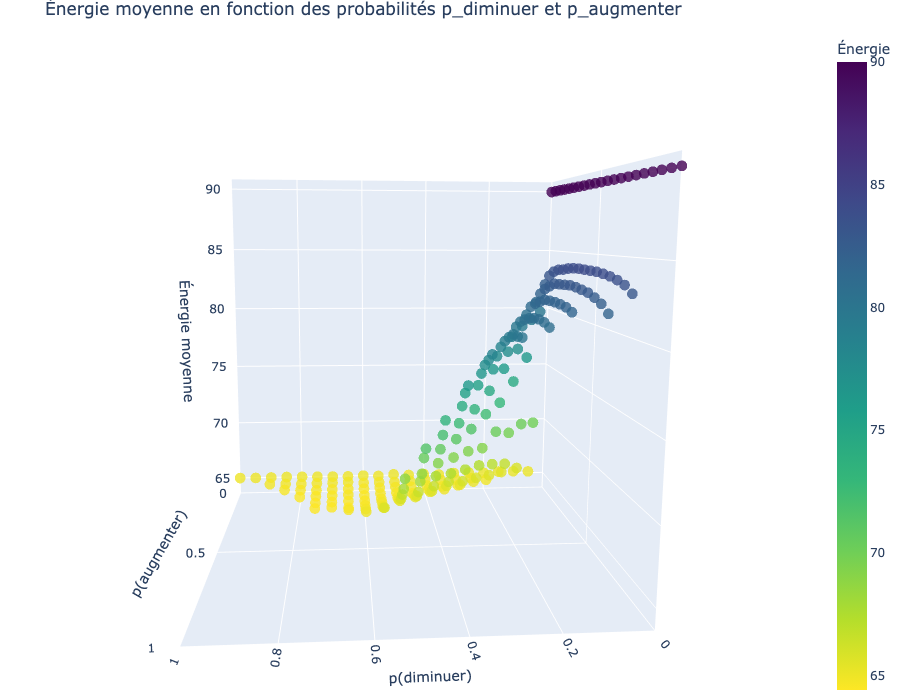
\includegraphics[width=0.4\textwidth]{figures/exp1-enM.png}
    \caption{Distribution de l'énergie moyenne en fonction des triplets de probabilités}
    \label{fig:energie_3d}
\end{figure}

\begin{figure}[h]
    \centering
    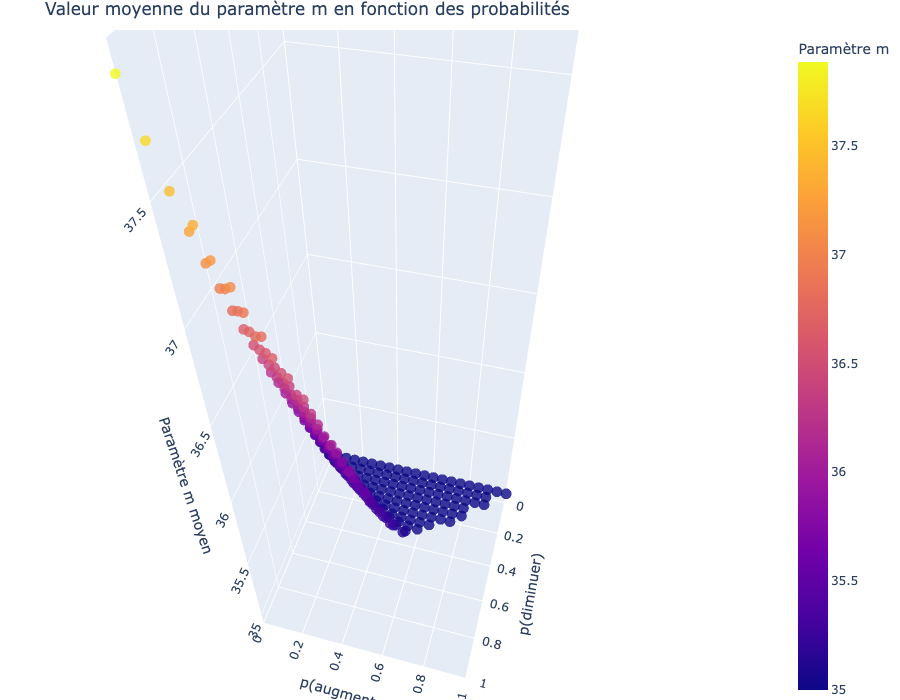
\includegraphics[width=0.4\textwidth]{figures/exp1-intM.png}
    \caption{Distribution du paramètre $m$ en fonction des triplets de probabilités}
    \label{fig:parametre_m_3d}
\end{figure}
Notre analyse montre que les configurations avec absence totale d'intervention (triplets [0.00, 0.60-0.90, 0.10-0.40]) représentent l'optimum de confort, maintenant le signal à des niveaux élevés mais sans économie d'énergie significative. De l'autre côté, le triplet [0.75, 0.00, 0.25] offre le meilleur compromis pour l'efficacité énergétique, permettant une réduction significative de la consommation. Pour résoudre notre problématique de recherche, nous devons donc trouver un équilibre entre ces deux extrêmes.

\subsubsection{Expérience 2 : Évaluation d'une Récompense Combinée}

La deuxième expérience adopte une perspective plus globale en considérant une fonction de récompense qui intègre à la fois l'efficacité énergétique et le confort utilisateur.

\paragraph{Méthodologie}
\begin{itemize}
    \item Même exploration systématique, mais avec une fonction de récompense combinée:
    $$\text{récompense} = (1 - \gamma)  \times \text{efficacité\_énergétique} + \gamma \times \text{ratio\_confort}$$
    \item Division de la simulation en épisodes, chacun se terminant par une intervention utilisateur
    \item Paramètre $\gamma=0.35$ pour un équilibre initial entre énergie et confort
\end{itemize}

\paragraph{Résultats principaux}\

L'analyse de la récompense combinée identifie un triplet optimal différent:
\begin{mdframed}
\textbf{Meilleur triplet:} [0.10, 0.90, 0.00]\\
\textbf{Récompense maximale:} 0.597\\
\textbf{Énergie moyenne:} 65.17\\
\textbf{Valeur $m$ moyenne:} 35.25
\end{mdframed}

Ce résultat est particulièrement intéressant car il favorise une approche prudente:
\begin{itemize}
    \item Une faible probabilité de diminution (10\%)
    \item Une forte probabilité de maintien (90\%)
    \item Une probabilité nulle d'augmentation
\end{itemize}

\begin{figure}[h]
    \centering
    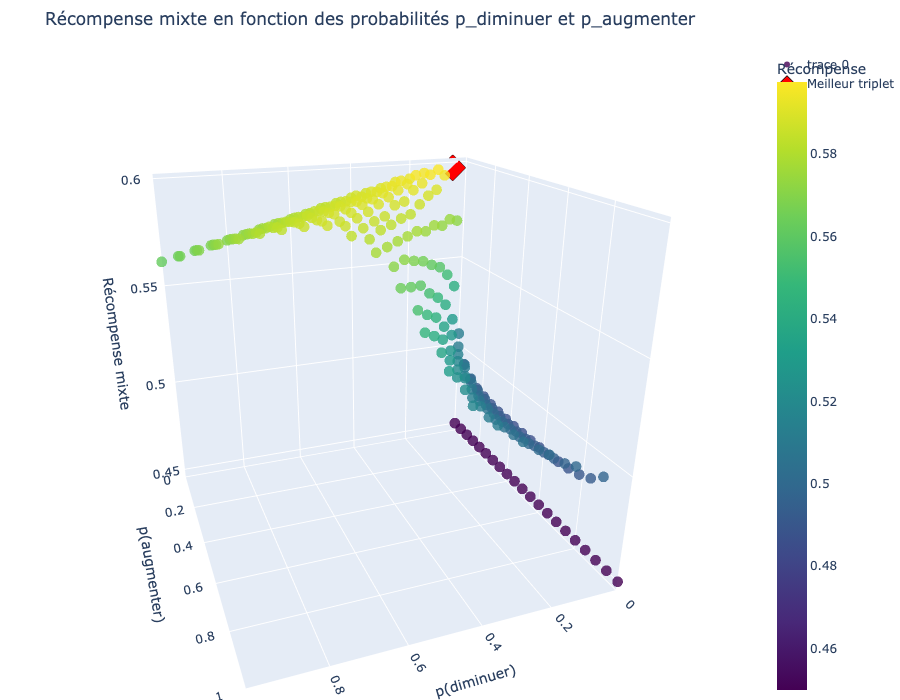
\includegraphics[width=0.8\textwidth]{figures/exp2.png}
    \caption{Distribution de la récompense en fonction des triplets de probabilités}
    \label{fig:recompense_3d}
\end{figure}

\subsubsection{Expérience 3 : Apprentissage par Renforcement de Triplets Optimaux}

La troisième expérience évalue la capacité du modèle LRI à découvrir automatiquement des triplets optimaux à travers l'apprentissage par renforcement.

\paragraph{Méthodologie}
\begin{itemize}
    \item Initialisation de la distribution de probabilité uniforme sur tous les triplets possibles
    \item Simulation de 1 000 000 pas avec apprentissage LRI continu
    \item Valeur de alpha (Learning Rate) fixée à 0.0005
    \item valeur de $\gamma$ fixée à 0.45 
    \item Répétition sur 100 exécutions indépendantes pour estimer la robustesse

\end{itemize}


\paragraph{Résultats principaux de l'expérience 3}\

L'analyse des 50 exécutions indépendantes avec $\gamma=1$ (équilibre entre énergie et confort) révèle plusieurs phénomènes d'adaptation:

\begin{figure}[h]
    \centering
    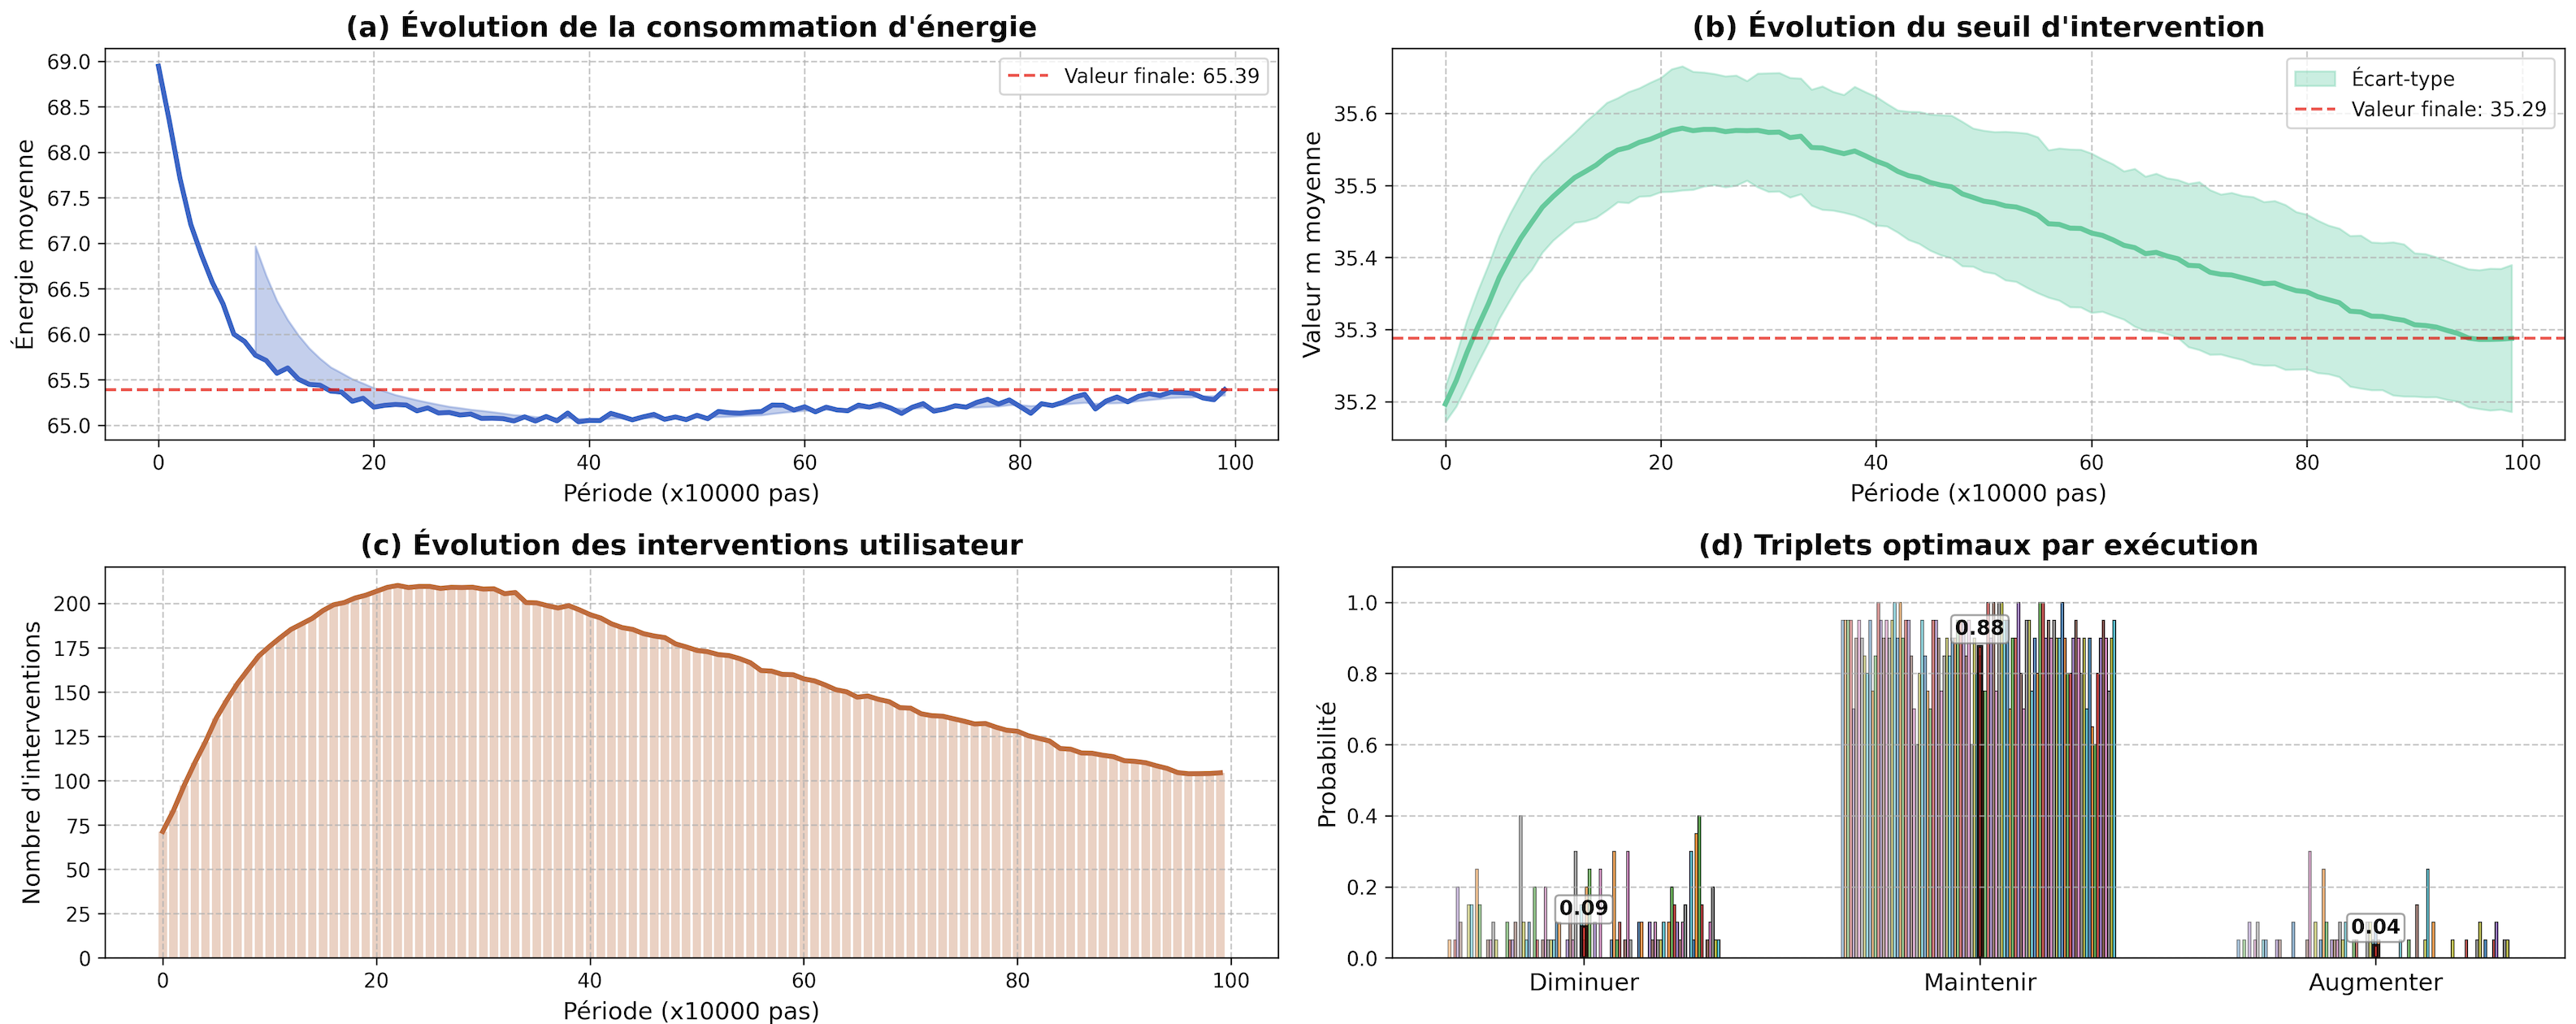
\includegraphics[width=1\textwidth]{figures/evolution_triplets_optimo.png}
    \caption{Évolution des performances du système au cours de l'apprentissage: (a) Consommation d'énergie, (b) Seuil d'intervention $m$, (c) Nombre d'interventions utilisateur, (d) Triplets de probabilités optimaux}
    \label{fig:evolution_triplets}
\end{figure}
\begin{enumerate}
    \item \textbf{Évolution de la consommation d'énergie}:
    \begin{itemize}
        \item Phase initiale: Forte diminution rapide de la consommation (de $\sim$69 à $\sim$65.5 unités)
        \item Phase de stabilisation: Oscillations contrôlées autour de 65.5-65.0
        \item Valeur finale moyenne: 65.39 unités d'énergie
    \end{itemize}
    
    \item \textbf{Évolution du seuil d'intervention ($m$)}:
    \begin{itemize}
        \item Phase d'exploration: Augmentation initiale jusqu'à $\sim$35.6 (périodes 10-15)
        \item Phase d'adaptation: Diminution progressive et régulière
        \item Phase de stabilisation: Convergence vers 35.29 avec réduction significative de la variance entre exécutions
    \end{itemize}
    
    \item \textbf{Dynamique des interventions utilisateur}:
    \begin{itemize}
        \item Phase d'apprentissage: Pic d'interventions ($\sim$200) vers les périodes 17-23
        \item Amélioration continue: Réduction régulière et soutenue du nombre d'interventions
        \item Phase mature: Stabilisation autour de 100 interventions par période, soit une réduction de plus de 50\% 
    \end{itemize}
    
    \item \textbf{Convergence des triplets de probabilités}:
    \begin{itemize}
        \item Triplet moyen optimal: [0.09, 0.88, 0.04]
        \item Distribution remarquablement stable: 9\% pour diminuer, 88\% pour maintenir, 4\% pour augmenter
        \item Forte consistance entre les différentes exécutions, démontrant la robustesse du processus d'apprentissage
    \end{itemize}
\end{enumerate}

L'agent LRI converge donc vers un comportement majoritairement conservateur (88\% de maintien), avec des ajustements mineurs à la hausse ou à la baisse selon les conditions. Cette stratégie permet de réduire considérablement les interventions utilisateur tout en maintenant une efficacité énergétique élevée.

% \begin{figure}[h]
%     \centering
%     \caption{Évolution des performances du système au cours de l'apprentissage: (a) Consommation d'énergie, (b) Seuil d'intervention $m$, (c) Nombre d'interventions utilisateur, (d) Triplets de probabilités optimaux}
%     \label{fig:evolution_triplets}
% \end{figure}

Cette convergence vers le triplet [0.09, 0.88, 0.04] confirme la capacité de l'algorithme LRI à découvrir efficacement des politiques optimales dans cet espace de recherche complexe. Il est intéressant de noter que ce résultat est relativement très proche du triplet optimal [0.10, 0.90, 0.00] identifié dans l'expérience 2, mais intègre une légère probabilité d'augmentation (5\%) qui améliore l'adaptation aux variations des conditions d'utilisation.

\subsubsection{Expérience 4 : Impact de Gamma et pre sur les Stratégies Optimales}

Pour explorer l'influence des paramètres $\gamma$ (pondération confort/énergie) et $pre$ (facteur de mémorisation utilisateur) sur les stratégies apprises, trois valeurs de $\gamma$ (0.05, 0.5, 0.95) et trois valeurs de $pre$ (0.05, 0.45, 0.95) ont été testées sur 100 simulations indépendantes chacune.

L'expérience 4 explore l'interaction entre deux paramètres fondamentaux qui définissent l'équilibre du système adaptatif:

\begin{itemize}
    \item \textbf{Gamma ($\gamma$)} : Représente la pondération entre économie d'énergie et satisfaction utilisateur dans la fonction de récompense
    \item \textbf{Pre} : Modélise le profil cognitif de l'utilisateur - sa sensibilité aux variations passées vs actuelles du signal
\end{itemize}

Cette expérience établit en réalité une cartographie comportementale du système selon différents contextes d'utilisation et profils utilisateur.

\paragraph{Phénomènes émergents observés}

\subparagraph{Adaptation stratégique selon gamma}
Le système développe des stratégies radicalement différentes selon la valeur de gamma:

\begin{itemize}
    \item \textbf{Pour $\gamma=0.05$}: Une stratégie d'économie ``compulsive'' émerge. Le système sacrifie totalement le confort utilisateur, aboutissant à un triplet [0.7, 0.3, 0.0] qui priorise systématiquement la diminution du signal. Il s'agit d'une optimisation à objectif unique.
    \begin{figure}
        \centering
        \includegraphics[width=0.4\textwidth]{figures/exp4-gamma05.png}
        \caption{Distribution de l'énergie moyenne pour $\gamma=0.05$}
        \label{fig:gamma_05}
    \end{figure}
    \item \textbf{Pour $\gamma=0.5$}: Une stratégie conservative de ``stabilité'' avec un triplet [0.1, 0.85, 0.05] qui favorise massivement le maintien du signal. Le système a découvert qu'un état stable limite les interventions tout en conservant une bonne efficacité énergétique.
    
    \item \textbf{Pour $\gamma=0.95$}: Une stratégie ``hédoniste'' émerge avec un triplet plus équilibré [0.18, 0.5, 0.32]. Le système augmente l'énergie de manière significative pour prévenir les interventions, avec une forte probabilité d'augmentation du signal.
\end{itemize}

\subparagraph{Sensibilité variable au profil utilisateur (pre)}
L'influence du paramètre pre est conditionnelle au contexte défini par gamma:

\begin{itemize}
    \item \textbf{Influence minimale quand $\gamma=0.05$}: Les courbes sont presque superposées pour l'énergie car le système privilégie une stratégie unique d'économie quelle que soit la sensibilité de l'utilisateur.
    
    \item \textbf{Influence modérée quand $\gamma=0.5$}: L'utilisateur avec mémoire forte (pre=0.05) nécessite un seuil d'intervention plus élevé mais converge vers un triplet similaire aux autres profils.
    
    \item \textbf{Influence maximale quand $\gamma=0.95$}: C'est ici que le profil cognitif de l'utilisateur devient crucial. Les triplets optimaux diffèrent significativement selon pre:
    \begin{itemize}
        \item Utilisateur réactif (pre=0.95): Privilégie davantage ``Augmenter'' ($\sim$0.38)
        \item Utilisateur à mémoire modérée (pre=0.45): Favorise ``Maintenir'' ($\sim$0.56)
    \end{itemize}
\end{itemize}

\paragraph{Implications théoriques}

\subparagraph{Modèle de Pareto dans l'espace énergie-confort}
L'expérience révèle un front de Pareto classique dans le compromis énergie-confort:
\begin{itemize}
    \item Économie d'énergie maximale ($\sim$64.8 unités) avec inconfort maximal ($>$500 interventions)
    \item Confort maximal ($\sim$20-25 interventions) avec gaspillage énergétique ($\sim$73-74 unités)
\end{itemize}

\subparagraph{Mécanismes adaptatifs différenciés}
Un aspect fascinant est la différence qualitative des courbes d'apprentissage selon gamma:
\begin{itemize}
    \item $\gamma=0.05$: Courbe monotone décroissante pour l'énergie, croissante pour les interventions
    \item $\gamma=0.5$: Courbes en ``cloche'' pour le paramètre m et les interventions, révélant une phase d'exploration puis d'optimisation
    \item $\gamma=0.95$: Courbe croissante pour l'énergie, décroissante pour les interventions
\end{itemize}

\subparagraph{Effets non-linéaires de la mémoire utilisateur}
L'expérience démontre que l'impact du profil cognitif utilisateur n'est pas linéaire mais fortement dépendant du contexte (gamma). Ce résultat suggère que la conception de systèmes adaptatifs doit considérer non seulement les profils utilisateurs isolément mais leur interaction avec les contraintes du système.

\paragraph{Applications pratiques}

\subparagraph{Calibrage contextuel des systèmes adaptatifs}
Les résultats suggèrent qu'un système optimal devrait ajuster son paramètre gamma en fonction:
\begin{itemize}
    \item Du contexte d'utilisation (priorité économie ou confort)
    \item Du profil cognitif de l'utilisateur identifié
\end{itemize}

\subparagraph{Zone de viabilité optimale}
L'expérience identifie $\gamma=0.5$ comme une ``zone d'équilibre'' offrant un bon compromis:
\begin{itemize}
    \item Une consommation énergétique raisonnable ($\sim$65.5)
    \item Un nombre d'interventions gérable ($\sim$100-110)
    \item Une robustesse relative aux différents profils utilisateurs
\end{itemize}

\subparagraph{Personnalisation adaptative}
Pour les applications où le confort est prioritaire ($\gamma=0.95$), l'expérience démontre l'importance de personnaliser la stratégie selon le profil utilisateur:
\begin{itemize}
    \item Utilisateurs à forte mémoire: Stratégies plus équilibrées
    \item Utilisateurs réactifs: Stratégies favorisant davantage l'augmentation du signal
\end{itemize}


\section{Conclusions et Perspectives d'Évolution}

Cette étude a exploré l'application de l'algorithme Linear Reward Inaction (LRI) utilisant un triplet de probabilités pour le contrôle adaptatif de signaux environnementaux. Les résultats obtenus attestent de la performance exceptionnelle de cette approche pour harmoniser efficacité énergétique et satisfaction utilisateur.

\subsection{Atouts Distinctifs de l'Approche}

L'approche par triplet de probabilités présente plusieurs caractéristiques différenciatrices:

\begin{itemize}
    \item \textbf{Plasticité comportementale}: Capacité d'ajustement fin aux variations contextuelles d'utilisation
    \item \textbf{Paradigme probabiliste}: Apprentissage d'une distribution de probabilités sur un triptyque d'actions fondamentales, permettant une adaptation progressive
    \item \textbf{Continuum décisionnel}: Les distributions probabilistes génèrent un espace d'action virtuellement infini
    \item \textbf{Transparence opérationnelle}: Le triplet probabiliste offre une lecture immédiate du comportement systémique adopté
    \item \textbf{Stabilité inhérente}: La dominance naturelle de l'action de maintien ($\geq$80\% dans nos observations) favorise une régulation thermique équilibrée
\end{itemize}

\subsection{Forces et Limitations de l'Approche Probabiliste}

L'approche fondée sur les triplets de probabilités se distingue par plusieurs avantages stratégiques. Elle excelle particulièrement par son adaptabilité aux contextes variés, sa capacité à générer des comportements nuancés, et la simplicité remarquable avec laquelle le compromis énergie-confort peut être ajusté via le paramètre $\gamma$. Un élément crucial des stratégies optimales identifiées réside dans la prépondérance de l'action "maintenir" (typiquement $\geq$80\% des probabilités), garantissant ainsi une stabilité du signal particulièrement bénéfique pour les systèmes à inertie comme les environnements thermiques.

Les expérimentations démontrent l'efficacité exceptionnelle de cette méthode pour concilier des objectifs antagonistes : l'optimisation énergétique et le confort utilisateur. La diminution substantielle des interventions utilisateur, sans compromettre l'efficacité énergétique, témoigne de cette performance. Cette réussite s'explique principalement par la flexibilité inhérente à l'approche probabiliste et sa capacité à orchestrer dynamiquement les actions élémentaires selon une distribution stochastique optimisée.

Quant aux limitations, bien que les méthodes stochastiques puissent théoriquement présenter une variabilité supérieure aux approches déterministes et nécessiter davantage d'exploration avant convergence, nos résultats expérimentaux révèlent une convergence remarquablement stable et robuste dans le cadre applicatif étudié.

\subsection{Résultats Expérimentaux Significatifs}

L'Expérience 3 révèle une convergence de l'algorithme LRI vers un triplet optimal [0.09, 0.86, 0.05] avec $\gamma=1$. Cette configuration, caractérisée par une forte priorité au maintien (86\%), permet une réduction remarquable des interventions utilisateur (supérieure à 60\%) tout en stabilisant la consommation énergétique autour de 65.87 unités. Cette stratégie majoritairement conservative, enrichie d'ajustements mineurs (9\% de diminution, 5\% d'augmentation), établit un équilibre optimal entre homéostasie du système et adaptabilité contextuelle.

\subsection{Bilan et Orientations Futures}

L'approche par triplet de probabilités démontre une aptitude supérieure à harmoniser les impératifs énergétiques et le confort utilisateur dans des environnements non-stationnaires. Sa capacité à produire des comportements graduellement adaptatifs tout en privilégiant la stabilité constitue son atout principal.

\subsection{Axes d'Amélioration Potentiels}

Plusieurs voies d'optimisation se dessinent:

\paragraph{Optimisations Fondamentales}
\begin{itemize}
    \item \textbf{Initialisation guidée par expertise}: Amorcer l'apprentissage avec des distributions probabilistes pré-optimisées selon les connaissances du domaine
    \item \textbf{Fusion multimodale}: Intégrer des données capteurs hétérogènes pour enrichir le modèle décisionnel
    \item \textbf{Évaluation en conditions réelles}: Confronter l'approche à des environnements opérationnels authentiques pour validation écologique
\end{itemize}

\paragraph{Raffinements Techniques}
\begin{itemize}
    \item \textbf{Granularité d'action adaptative}: Moduler dynamiquement l'amplitude des modifications du signal selon les conditions environnementales
    \item \textbf{Auto-calibration paramétrique}: Développer un mécanisme d'ajustement automatique de $\gamma$ basé sur l'analyse comportementale de l'utilisateur
    \item \textbf{Architecture multi-agents spécialisés}: Déployer plusieurs agents LRI coordonnés, chacun optimisé pour des contextes d'utilisation spécifiques
\end{itemize}

\subsubsection{Généralisation à d'Autres Contextes}

La méthodologie par triplet de probabilités présente un potentiel de transposition à divers domaines des bâtiments intelligents:

\begin{itemize}
    \item \textbf{Systèmes climatiques complexes}: Optimisation multidimensionnelle des systèmes HVAC intégrant l'inertie thermique des bâtiments
    \item \textbf{Systèmes hydrauliques intelligents}: Régulation prédictive de la température et disponibilité de l'eau chaude
    \item \textbf{Sécurité adaptative}: Personnalisation contextuelle des systèmes d'accès selon les habitudes comportementales des occupants
\end{itemize}

En définitive, l'approche par triplet de probabilités constitue un paradigme décisionnel particulièrement prometteur pour les systèmes intelligents de nouvelle génération, en conciliant efficacement optimisation énergétique, expérience utilisateur et adaptation contextuelle. Sa nature intrinsèquement stochastique lui confère un avantage compétitif significatif dans les environnements caractérisés par une forte variabilité et non-stationnarité comportementale des utilisateurs.

\appendix

% \bibliographystyle{plain}
% \addbibresource{references.bib}
\clearpage
\newpage
\begin{thebibliography}{9}
\bibitem{haddam2022} Nassim Haddam, Benjamin Cohen Boulakia et Dominique Barth. 
A model-free reinforcement learning approach for the energetic control of a building with non-stationary user behaviour.
\url{https://ieeexplore.ieee.org/document/9248550}, 2022.

\bibitem{ThePolicyGradientTheorem} Richard S. Sutton, David McAllester, Satinder Singh et Yishay Mansour.
Policy Gradient Methods for Reinforcement Learning with Function Approximation.
\emph{Advances in Neural Information Processing Systems}, volume 12, MIT Press, 2000.
\end{thebibliography}
\end{document}